\section{Introduction}

Language plays a fundamental role in facilitating communication and self-expression for humans, and likewise, communication holds paramount importance for machines in their interactions with humans and other systems. Large Language Models (LLMs) have emerged as cutting-edge artificial intelligence systems designed to process and generate text, aiming to communicate coherently~\cite{y2022large}. The need for LLMs stems from the growing demand for machines to handle complex language tasks, including translation, summarization, information retrieval, and conversational interactions. 
Recently, significant breakthroughs have been witnessed in language models, primarily attributed to deep learning techniques, advancements in neural architectures like transformers, increased computational capabilities, and the accessibility of training data extracted from the internet~\cite{chernyavskiy2021transformers}. These developments have brought about a revolutionary transformation by enabling the creation of Large Language Models (LLMs) that can approximate human-level performance on certain evaluation benchmarks~\cite{wang2019superglue,adiwardana2020towards}. 


\begin{figure}[tbp]
\centering
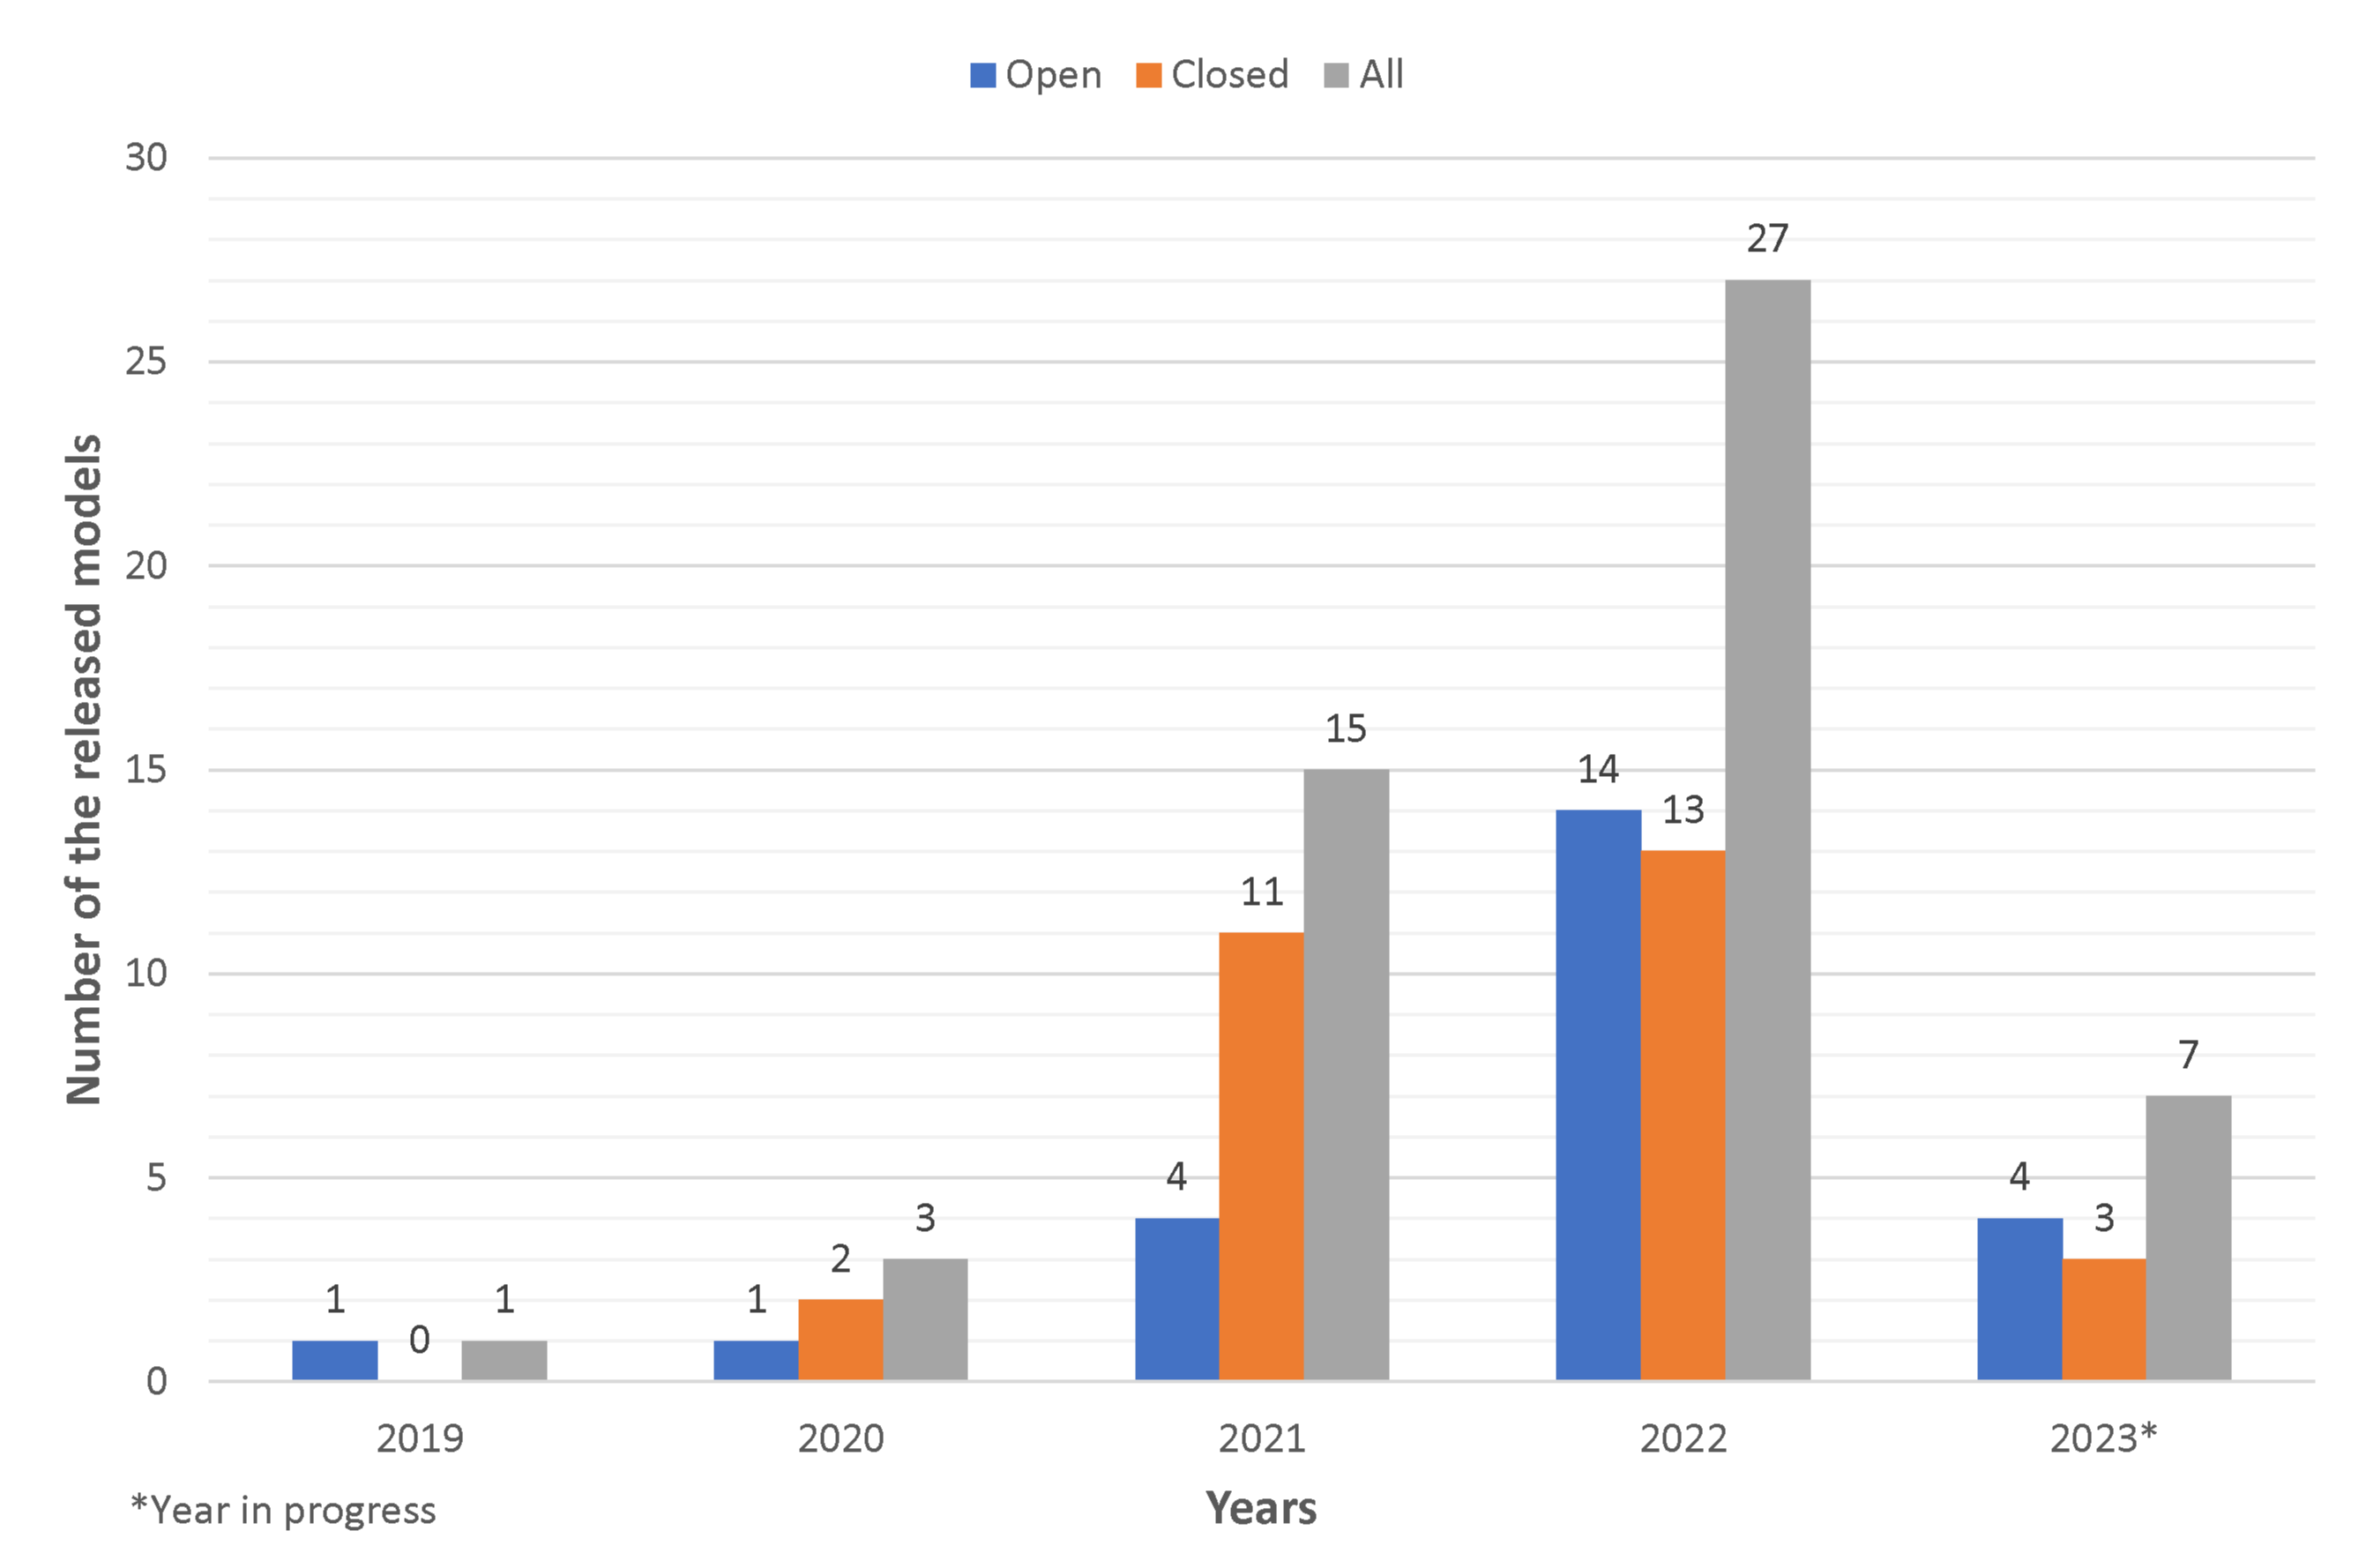
\includegraphics[width=1\columnwidth]{Figure/Column_Chart.png}
\caption{The trends in the number of LLM models introduced over the years.}
%\caption{Number of LLMs introduced over the years.}
\label{fig:num_LLMs_barchart}
\end{figure}

\begin{figure*}[tbp]
\centering
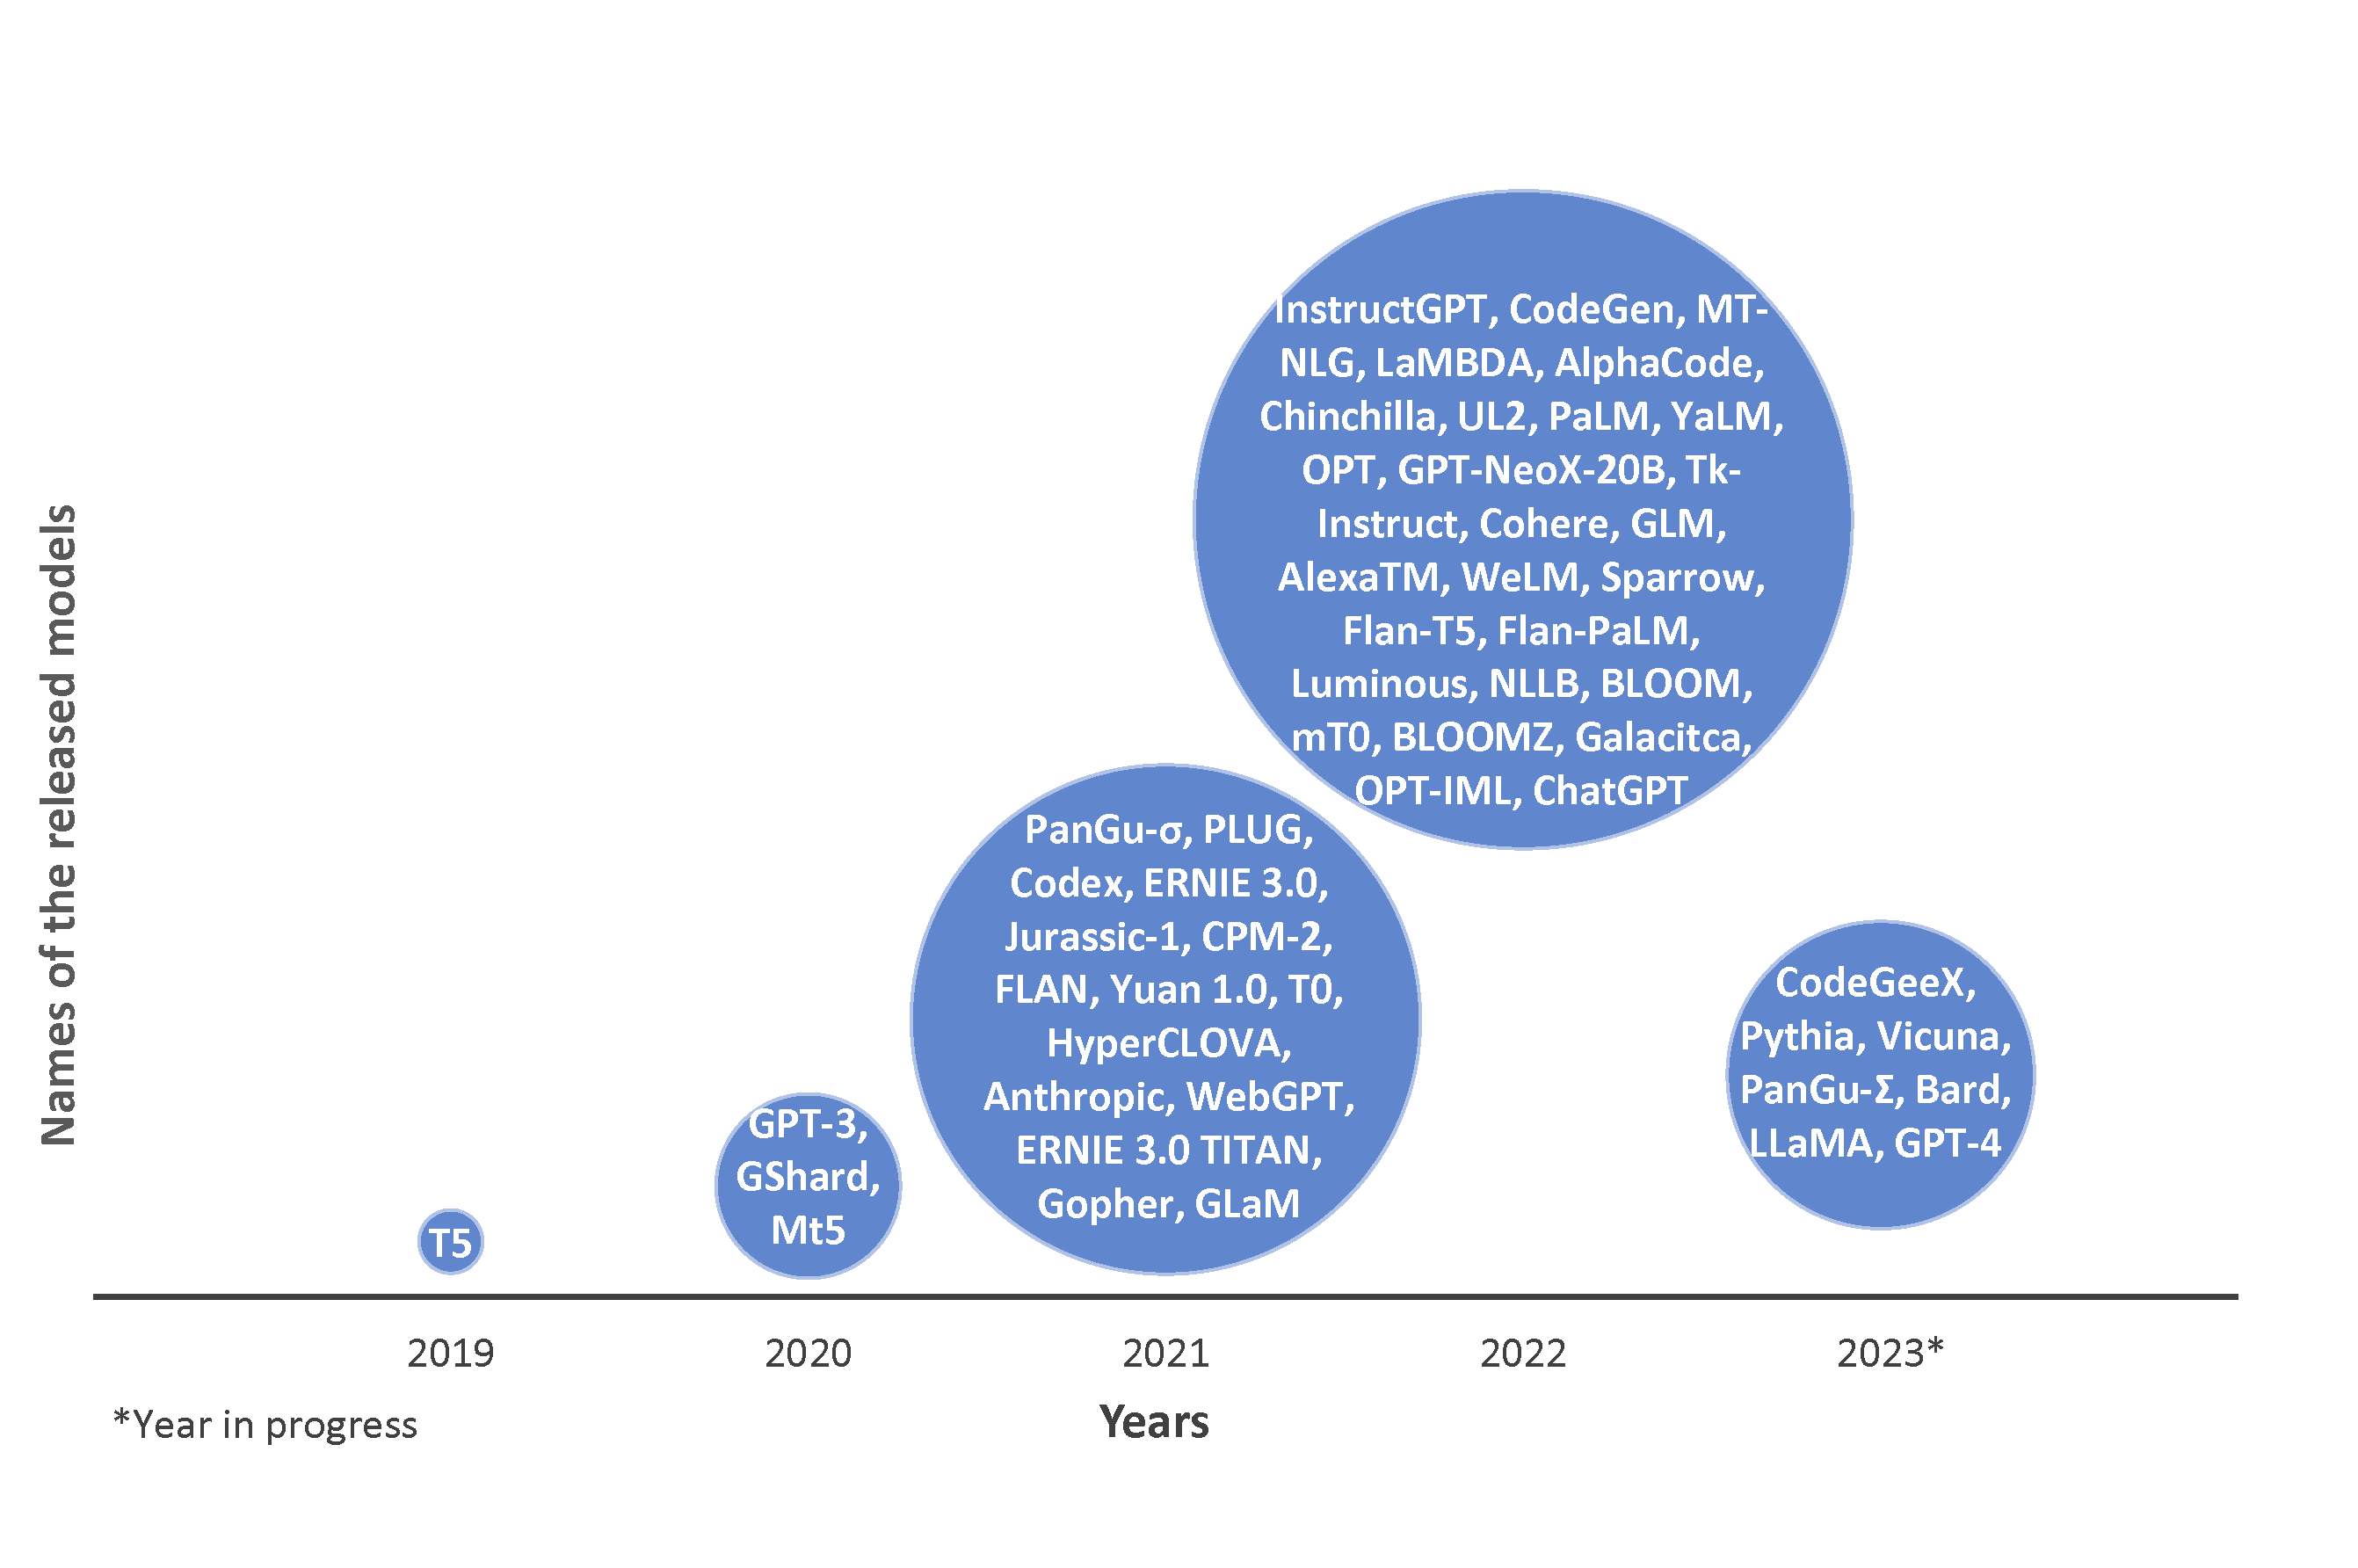
\includegraphics[width=2\columnwidth]{Figure/Bubble_Chart.png}
\caption{The progressive introduction of LLM models demonstrates advances in natural language processing explicitly adapted to various fields and provides increased research,  analysis, and application capabilities.}
%\caption{LLMs introduced over the years.}
\label{fig:LLMs_bubblechart}
\end{figure*}

LLMs, particularly pre-trained language models (PLM), have shown tremendous generalization abilities for text understanding and generation tasks while trained in a self-supervised setting on a large corpus of text~\cite{Bert, ELMO, BART}. The performance of pre-trained language models (PLMs) improves significantly when fine-tuned for downstream tasks, surpassing the performance of models trained from scratch. These characteristics of language models motivated researchers to train larger PLMs on even bigger datasets and found that scaling model and dataset size further improve the generalization abilities. 

Now modern LLMs are capable of performing various tasks like code generation, text generation, tool manipulation, reasoning, and understanding in zero-shot and few-shot settings in diverse domains, even without requiring any fine-tuning on downstream tasks~\cite{GPT-3, BLOOM, OPT}. Such generalization was previously unattainable with smaller models, marking a significant advancement in language modeling. This development has sparked enthusiasm and excitement within the research community for the enhancement of LLM architectures and training strategies, leading to the development of numerous LLMs~\cite{T5, mT5, CPM-2, GPT-3, BLOOM, OPT, PaLM}. 

% The graph~\ref{fig:num_LLMs_barchart} illustrates a growing trend in the number of released LLMs, including open-source and closed-source models, over the years.

The graph presented in Fig~\ref{fig:num_LLMs_barchart} depicts an increasing trend in the number of released LLMs, including open-source and closed-source models, over the years. Furthermore, Fig~\ref{fig:LLMs_bubblechart} highlights the names of significant releases of various LLMs.



% In recent years, pre-trained language models (PLM) have shown tremendous generalization abilities for text understanding and generation tasks while being trained in a self-supervised setting on a large corpus~\cite{Bert, ELMO, BART}. PLMs perform better when fine-tuned for downstream tasks as compared to the models trained from scratch. These characteristics of language models motivated researchers to train larger PLMs on even bigger datasets and found scaling model and dataset size further improve the generalization abilities. These huge models are given the name Large Language Models (LLMs).  \\
% LLMs are capable to perform diverse tasks like code generation, text generation, tool manipulation, reasoning, and understanding in zero-shot and few-shot settings in diverse domains, without requiring any fine-tuning on downstream tasks~\cite{GPT-3, BLOOM, OPT}. Such a generalized capacity was not possible with smaller models. This created a spark in the research community to propose better LLMs architectures and training strategies leading to the development of numerous LLMs~\cite{T5, mT5, CPM-2, GPT-3, BLOOM, OPT, PaLM}.   \\




During the early days of Large Language Models (LLMs), many research efforts focused on developing models for transfer learning to downstream tasks ~\cite{T5, mT5, UL2} until the emergence of models like GPT-3~\cite{GPT-3}, which demonstrated impressive performance even without fine-tuning. Due to the closed-source nature of GPT-3, there was a demand for open-source alternatives, leading to the development of various models ~\cite{BLOOM, OPT} operating at the scale of GPT-3 and trained on extensive web-based datasets~\cite{Common_Crawl,Wikipedia,Openwebtext_Dataset,BQ_Dataset}.   Subsequently, researchers proposed several architectural designs and training strategies that showed superior performance compared to GPT-3 across various tasks ~\cite{UL2, PaLM, U-PaLM, mtnlg}. 

The performance of LLMs improves further with instruction fine-tuning, outperforming pre-trained LLMs on various benchmarks~\cite{T0, mT0andBLOOMZ}. Instruction fine-tuning of LLMs refers to a specific training approach by incorporating additional prompts or instructions during the fine-tuning phase to guide the output and thus enable the users to have more fine-grained control over the outputs of LLMs. These prompts can be natural language instructions or example demonstrations based on the task's requirement. In the literature, different datasets have been curated for instruction fine-tuning. These datasets include more instances and tasks that further improve the performance over baselines~\cite{OPT_IML,mT0andBLOOMZ,Flan,Tk-INSTRUCT}. When performing instruction fine-tuning, all the model parameters need to be updated. However, parameter-efficient fine-tuning takes a different approach by updating only a small number of parameters while still maintaining good performance. This method keeps the original model frozen and adds a few extra parameters at different locations within the model~\cite{LMAdapted, LMAdapter_2, LMAdapter_3, Prompt_Tuning, Prefix_Tuning}. This approach helps achieve efficient fine-tuning while minimizing the impact on the model's overall performance.
% Instruction-tuning requires updating all the parameters. Compared to this, parameter-efficient fine-tuning updates only a small number of parameters without dropping the performance significantly. In this method, the original model is kept frozen and fewer additional parameters are added to the model at different positions as given in~\cite{LMAdapted, LMAdapter_2, LMAdapter_3, Prompt_Tuning, Prefix_Tuning}.  



The literature presents numerous pre-trained and fine-tuned models for LLMs with diverse approaches. Some survey papers provide an overview of augmented techniques in LLMs~\cite{survey_1}. Additionally, a comprehensive review is available that covers architectures, fine-tuning, emergent abilities, and the usability of LLMs~\cite{Survey_LLM}. Another survey provides a historical account of foundation models~\cite{survey_2}. However, these review papers do not delve into the specific details of individual models, offering only a surface-level understanding of architectures and training methods. In contrast, our paper aims to provide a more in-depth analysis of individual LLMs by discussing fine-grained details.


The absence of comprehensive and detailed discussions, particularly from a historical standpoint, regarding the architecture, training datasets, and other granular aspects of Large Language Models (LLMs), has motivated us to undertake an exhaustive survey. This survey aims to provide an in-depth and comprehensive analysis of LLMs, delving into the details surrounding their development, architecture, training datasets, and related components.
\begin{itemize}
\item To the best of our knowledge, this is the first comprehensive survey paper that discusses fine-grained details of LLMs. 
%Write about our survey and the contributions etc
\item We provide a thorough analysis of the existing literature regarding various LLMs architectures
and their categorization. Moreover, we also discussed the basics of the LLMs to make the paper self-sufficient and productive for the reader not familiar with LLMs.

% \item We have also identified future research directions that might help researchers to further enhance the methods and achieve new state-of-the-art.



\item Our paper focuses on providing comprehensive details for each LLM model and covers aspects such as architecture modifications, training objectives, datasets used, strategies for stable training, key findings, suggestions, and challenges encountered during training.

\item We aim to summarize these crucial details in our paper to assist researchers in identifying better architectures and training approaches for their work.
\end{itemize}


% Our paper focuses on providing comprehensive details for each LLM model and covers aspects such as architecture modifications, training objectives, datasets used, strategies for stable training, key findings, suggestions, and challenges encountered during training.
Our paper complements a recent survey paper~\cite{Survey_LLM} on LLMs that covers topics like data preprocessing, data cleaning, scaling laws, emergent abilities, adaptation tuning, and utilization. While the survey paper provides information on architectures, it does not delve into the fine-grained details of architectural changes, training objectives, and specific findings from proposed LLMs. 
% For every LLM, we provide details on changes in architecture, training objective, datasets, and strategies to stable training, findings and suggestions by every LLM, and other issues faced during training. Our paper complements a recent survey paper on LLMs that explains various topics on data preprocessing, data cleaning, scaling laws, emergent abilities, adaptation tuning, and utilization. It also provides information on architectures but does not discuss fine details on architectural changes, training objectives and findings of proposed LLMs. We summarize these details in this paper with the aim to help researchers in identifying better architectures and training approaches in their research work.    \\
We discuss LLMs model with a minimum of 10 billion parameters or more similar to the paper~\cite{Survey_LLM}. Models smaller than this scale are not discussed in our paper. One can refer to review papers such as~\cite{survey_smaller_LLMs_1, survey_smaller_LLMs_2, survey_1} for exploring smaller models.


% Similar to the paper~\cite{Survey_LLM}, our definition of LLM is a model with at-least 10B or more parameters. We do not discuss models smaller than the 10B scale. One can see a review of these smaller models in~\cite{survey_smaller_LLMs_1, survey_smaller_LLMs_2, survey_1}. \\
     

The organization of this paper is as follows. Section~\ref{sec:Background} discusses the background of LLMs, offering a concise overview of the essential building blocks that constitute these models. We discuss architectural styles, fine-tuning strategies, libraries, and distributed training methods. This section serves as a foundation for understanding the subsequent discussions on LLMs. Section~\ref{sec_review} focuses on LLMs overview, architectures, and training pipelines and strategies. Section~\ref{sec:Findings} presents the key findings derived from each LLM. Section~\ref{Model_Configurations_} highlights the configuration and parameters that play a crucial role in the functioning of these models. The LLM training and evaluation benchmarks are discussed in section~\ref{Datasets_and_Evaluation_}, followed by concluding remarks and future direction in the conclusion section.